\documentclass{article}
\usepackage[utf8]{inputenc}
\usepackage[T1]{fontenc}
\usepackage{graphicx}
\usepackage{amsmath}
\usepackage{wrapfig}
\usepackage[top=1in, bottom=1.25in, left=1.1in, right=1.1in]{geometry}

\title{Reporte - Evaluación 2}
\author{García Monge Itzel Alexia}
\date{26 de Abril, 2018}


\begin{document}
\maketitle

\section{Introducción}

El siguiente reporte resume la evaluación 2 del curso de \textit{Física Computacional I} del curso \textit{2018-1}, el cuál se centró en el atractor o sistena de Lorenz, encontrado por E. Lorens en 1963. El sistema de Lorenz fue el primer sistema de tres dimensiones autónomo en el cuál podía encontrarse un atractor caótico, recibiendo este atractor el famoso nombre de \textit{La mariposa de Lorenz}.



\section{Gráficas de Visualización del Atractor de Lorenz}


\subsection{Visualización y Animación 1}

Tomamos el código de visualización y animación de Geoff Boeing sobre el atractor de Lorenz, copiándolos en dos diferentes archivos \textbf{.ipynb} respectivamente y haciendo las modificaciones necesarias para que opere sin errores ni advertencias. En el código se integran los diferenciales que utilizando \textit{odient}, tomando los valores de los parámetros como $\sigma=10.0, \beta=\frac{8.0}{3.0}$ y $\rho=28.0 $. 

La gráfica de la solución del atractor de Lorenz con los parámetros establecidos siendo:

	\begin{center}
    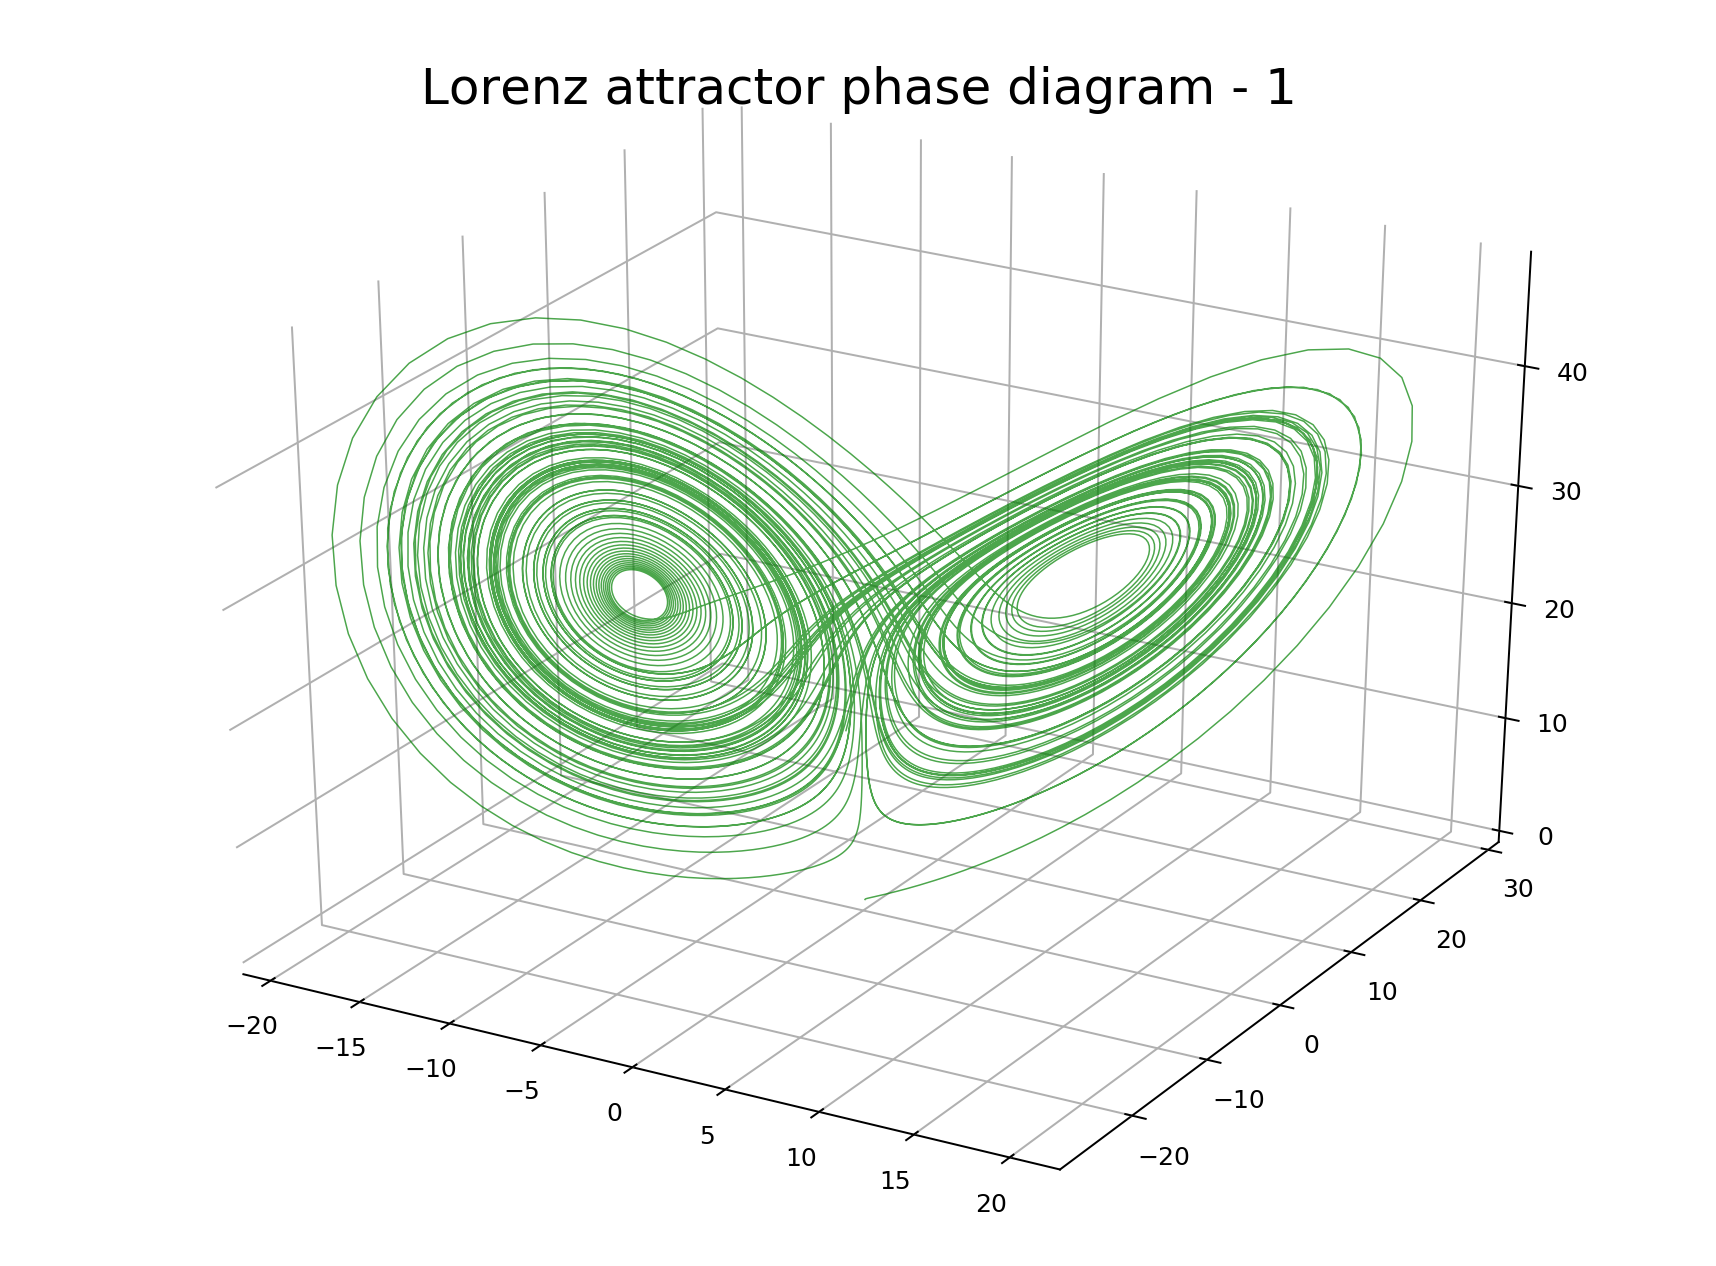
\includegraphics[height=7cm]{L-A-3d1.png}
    \end{center}

Si se deseara observar la gráfica del retrato de fase de manera bidimensional, se obtendría más de una gráfica, pues los ejes se alternarían para poder apreciar todas sus fases en diferentes posiciones.

	\begin{center}
    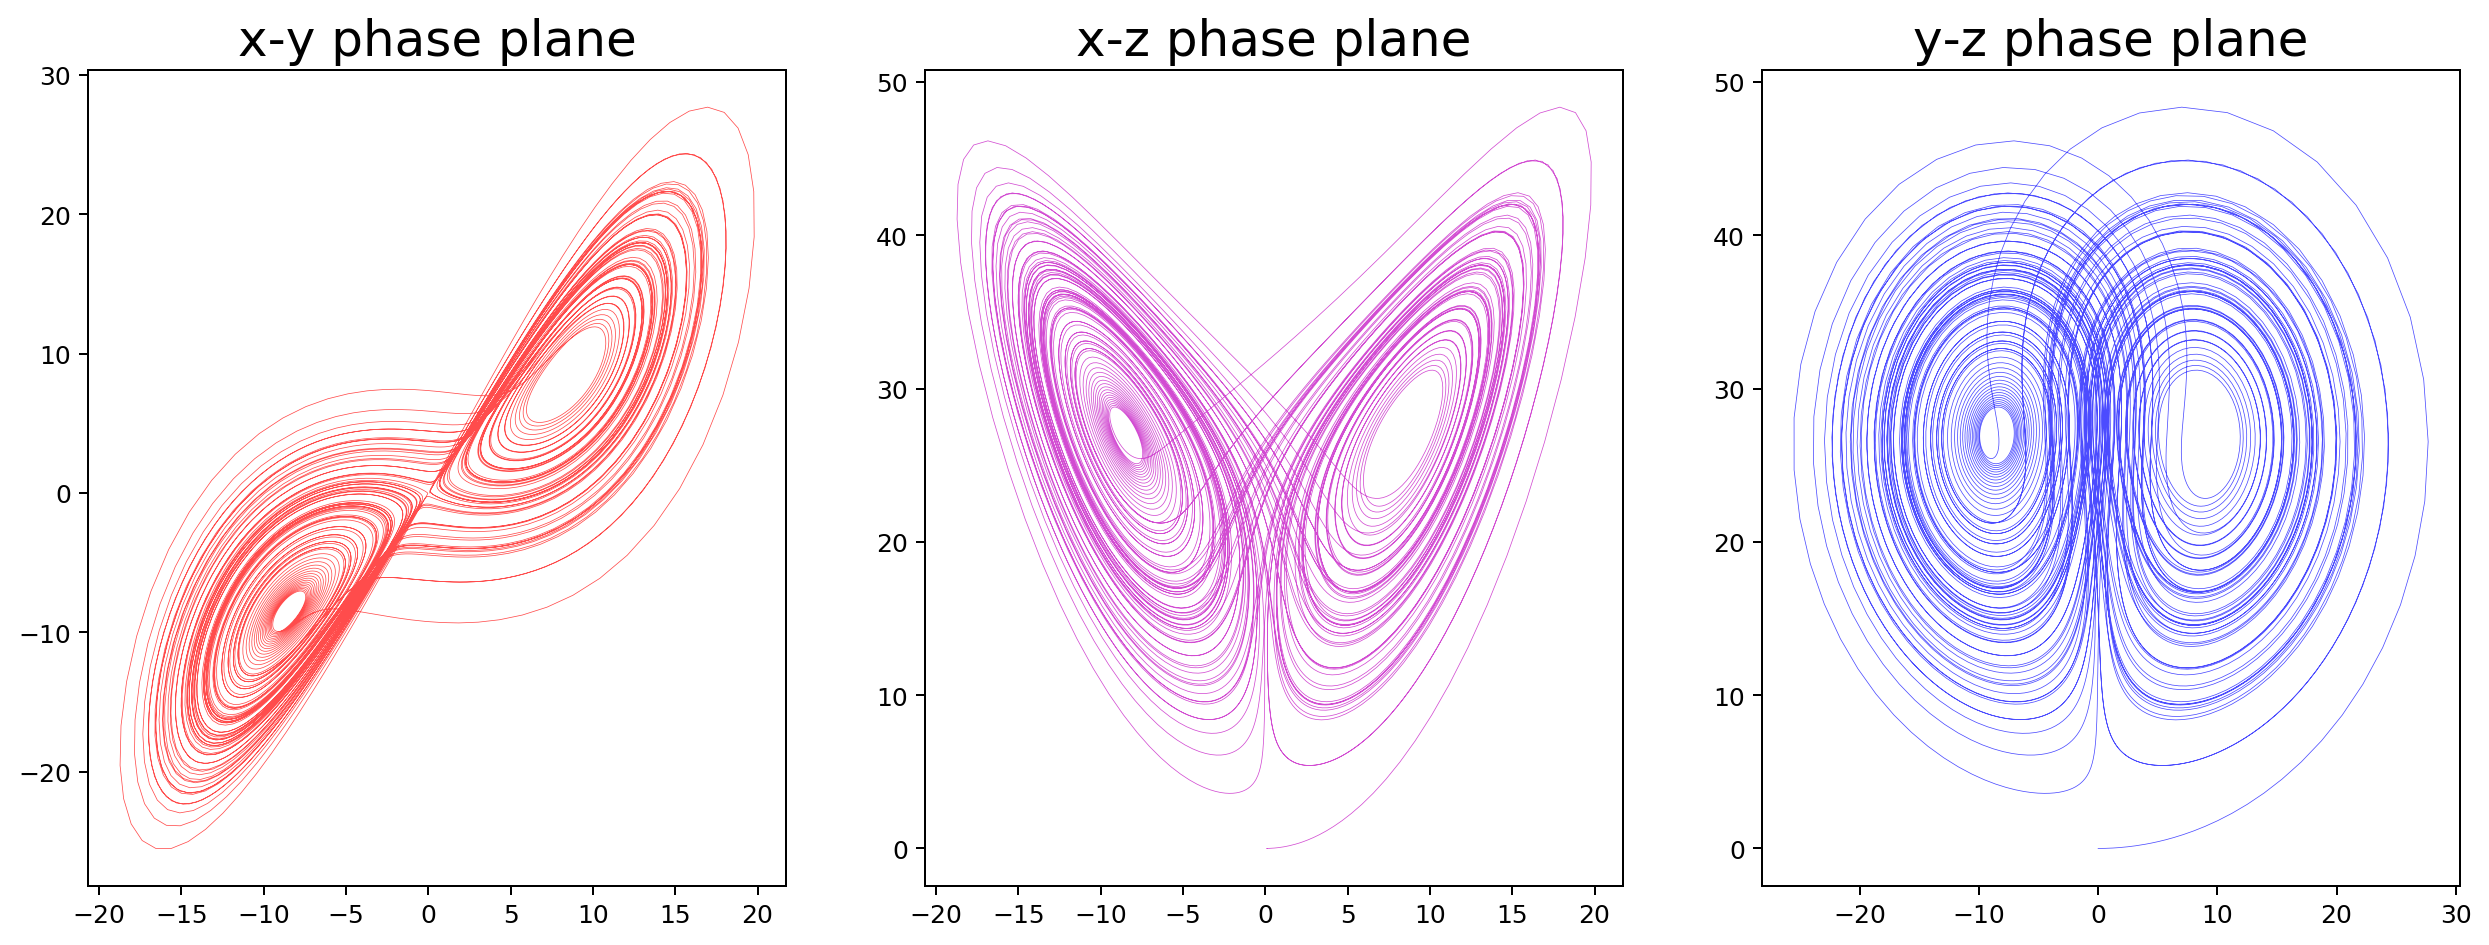
\includegraphics[height=5cm]{lorenz-attractor-phase-plane1.png}
    \end{center}

Mientras que el comportamiento de cada variable de posición \textit{x(t), y(t), z(t)} con respecto al tiempo-bajando del plano de tres dimensiones a un plano de dos dimensiones-para un atractor de Lorenz se comporta de forma distinta. La variable \textit{x(t)} representada con azul, \textit{y(t)} con rosa, y \textit{z(t) con cyan}.

	\begin{center}
    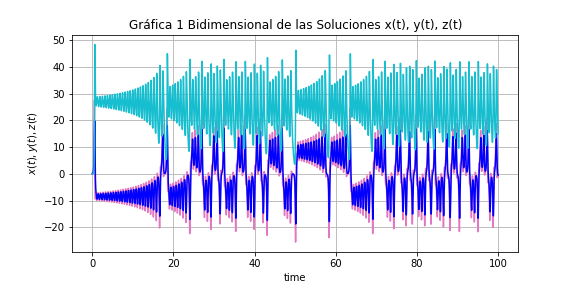
\includegraphics[height=5cm]{2_graficas1.png}
    \end{center}

En la \textit{Figura 2} es difícil observar una diferencia entre \textit{x(t)} y \textit{y(t)}, así que creamos un zoom con un intervalo de tiempo más pequeño para apreciar a mayor detalle sus posiciones, encontrando:
	
    \begin{center}
    \centering
    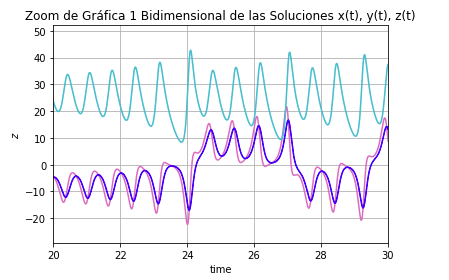
\includegraphics[height=5cm]{2_zoom1.png}
    \end{center}

Cada gráfica de posición contra el tiempo también puede apreciarse por separado:

	\begin{center}
    \centering
    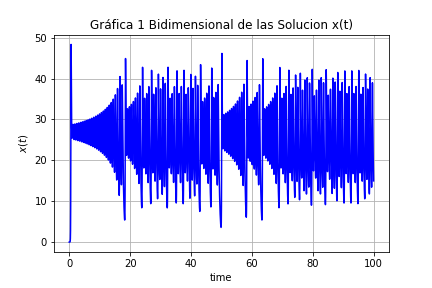
\includegraphics[height=5cm]{2_graficax.png}
	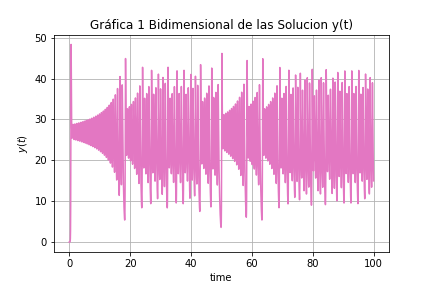
\includegraphics[height=5cm]{2_graficay.png}
    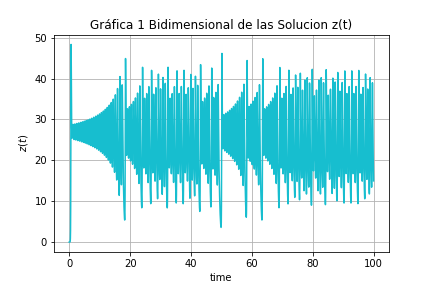
\includegraphics[height=5cm]{2_graficaz.png}
    \end{center}

Por otro lado, la animación creada-así como las demás animaciones que se crearon a lo largo del reporte-sólo podrán verse en el repositorio Github que le corresponde bajo el nombre de la Carpeta \textit{Evaluacion2}.




\section{Visualización y Animación 2}

Para la segunda visualización y animación se modificaron los valores de los parámetros, cambiando sus valores por $\sigma=28.0, \beta=4.0$ y $\rho=46.92 $.

Se puede observar como esta gráfica de la solución del atractor de Lorenz con los parámetros establecidos no cambia radicalmente con respecto a la primera gráfica creada:

	\begin{center}
    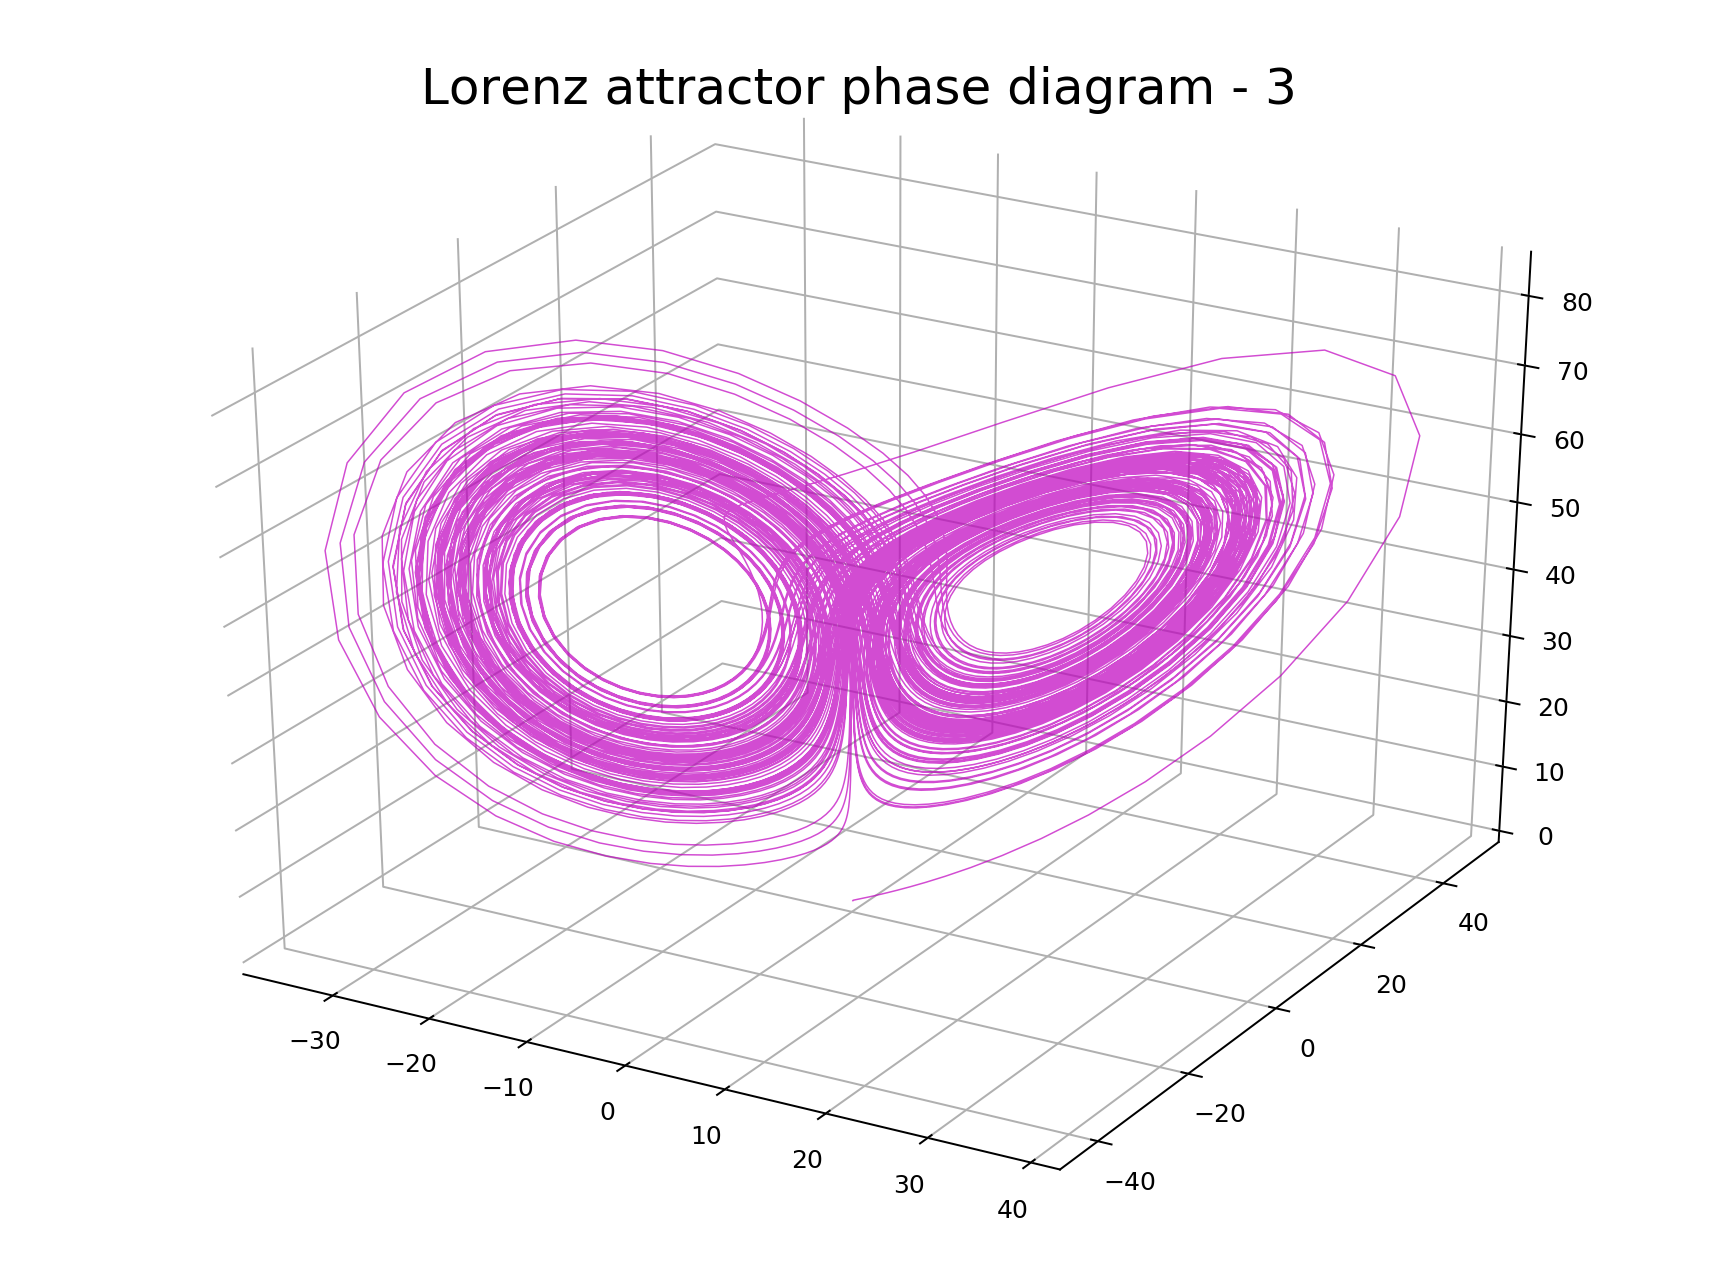
\includegraphics[height=7cm]{L-A-3d3.png}
    \end{center}

Las gráficas del retrato de fase de manera bidimensional son:

	\begin{center}
    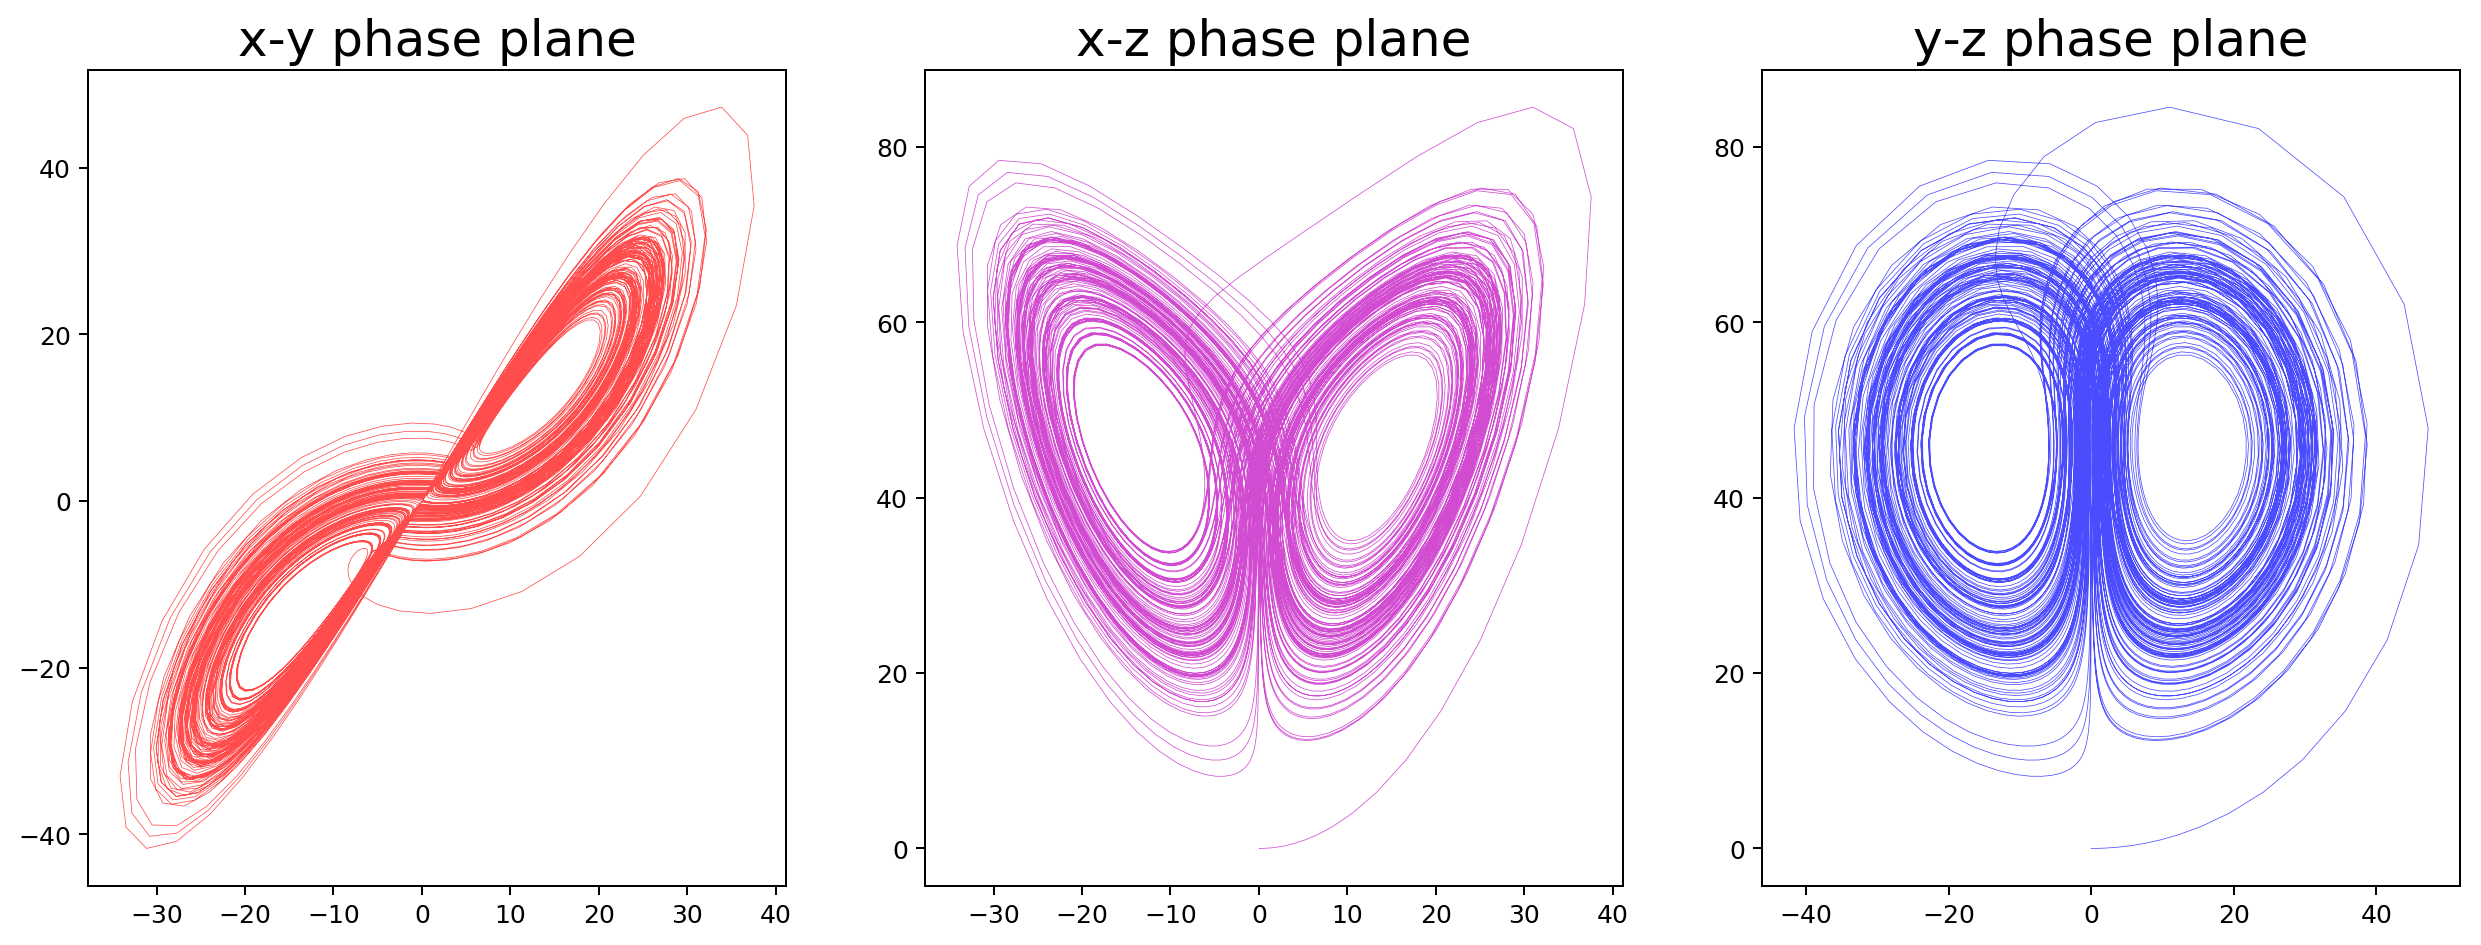
\includegraphics[height=5cm]{lorenz-attractor-phase-plane3.png}
    \end{center}

El comportamiento de cada variable de posición \textit{x(t), y(t), z(t)} con respecto al tiempo, sin cambiar la relación de variable-color con las gráficas anteriores:

	\begin{center}
    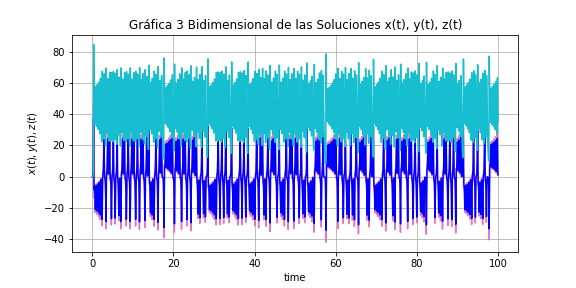
\includegraphics[height=5cm]{2_graficas3.png}
    \end{center}

Nuevamente, se presenta un problema en distinguir el comportamiento entre \textit{x(t)} y \textit{y(t)}, por lo que se hace un acercamiento:

    \begin{center}
    \centering
    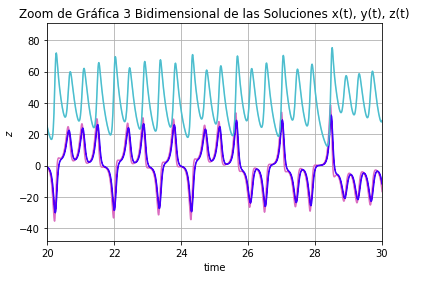
\includegraphics[height=5cm]{2_zoom3.png}
    \end{center}

Cada gráfica del comportamiento de la posición contra el tiempo por separado:

	\begin{center}
    \centering
    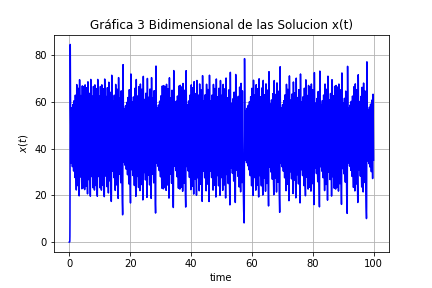
\includegraphics[height=5cm]{2_graficax3.png}
	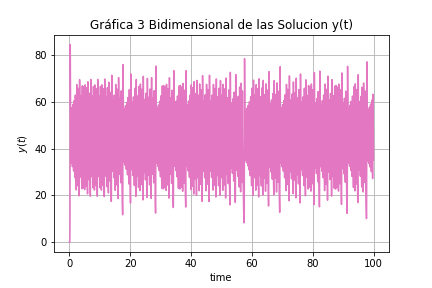
\includegraphics[height=5cm]{2_graficay3.png}
    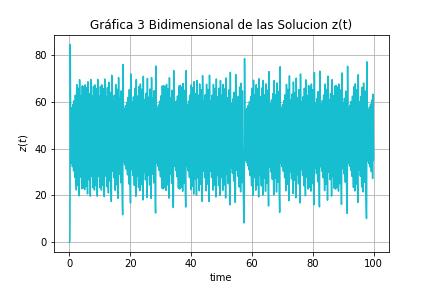
\includegraphics[height=5cm]{2_graficaz3.png}
    \end{center}



\section{Visualización y Animación 3}

En la tercera y última visualización los parámetros cambian de la forma $\sigma=10.0, \beta=\frac{8.0}{3.0}$ y $\rho=99.96 $.

A diferencia de la gráfica 2, aquí es posible encontrar que la gráfica de la solución del atractor de Lorenz con los nuevos parámetros establecidos cambia su forma con respecto a la primera y segunda gráfica creada:

	\begin{center}
    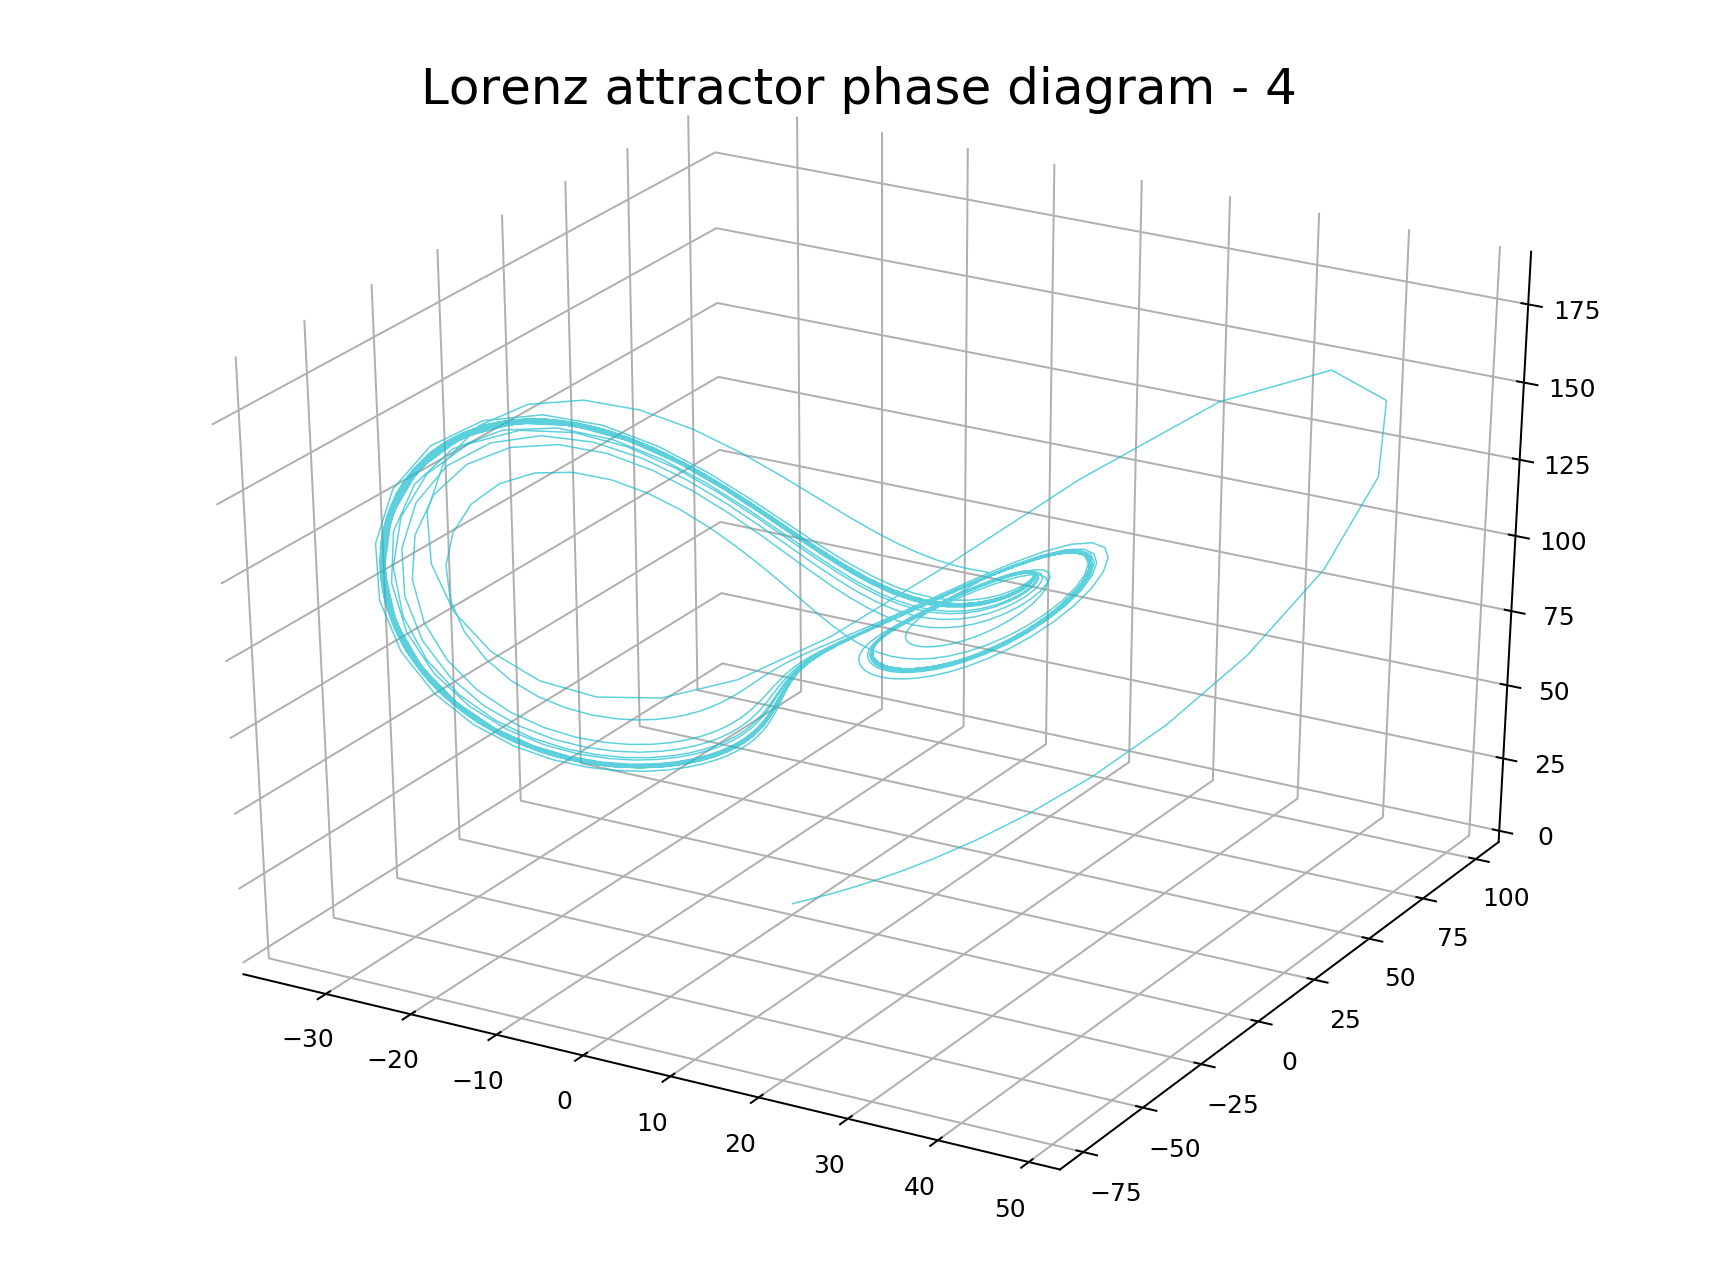
\includegraphics[height=7cm]{L-A-3d4.png}
    \end{center}

Las gráficas del retrato de fase de manera bidimensional son:

	\begin{center}
    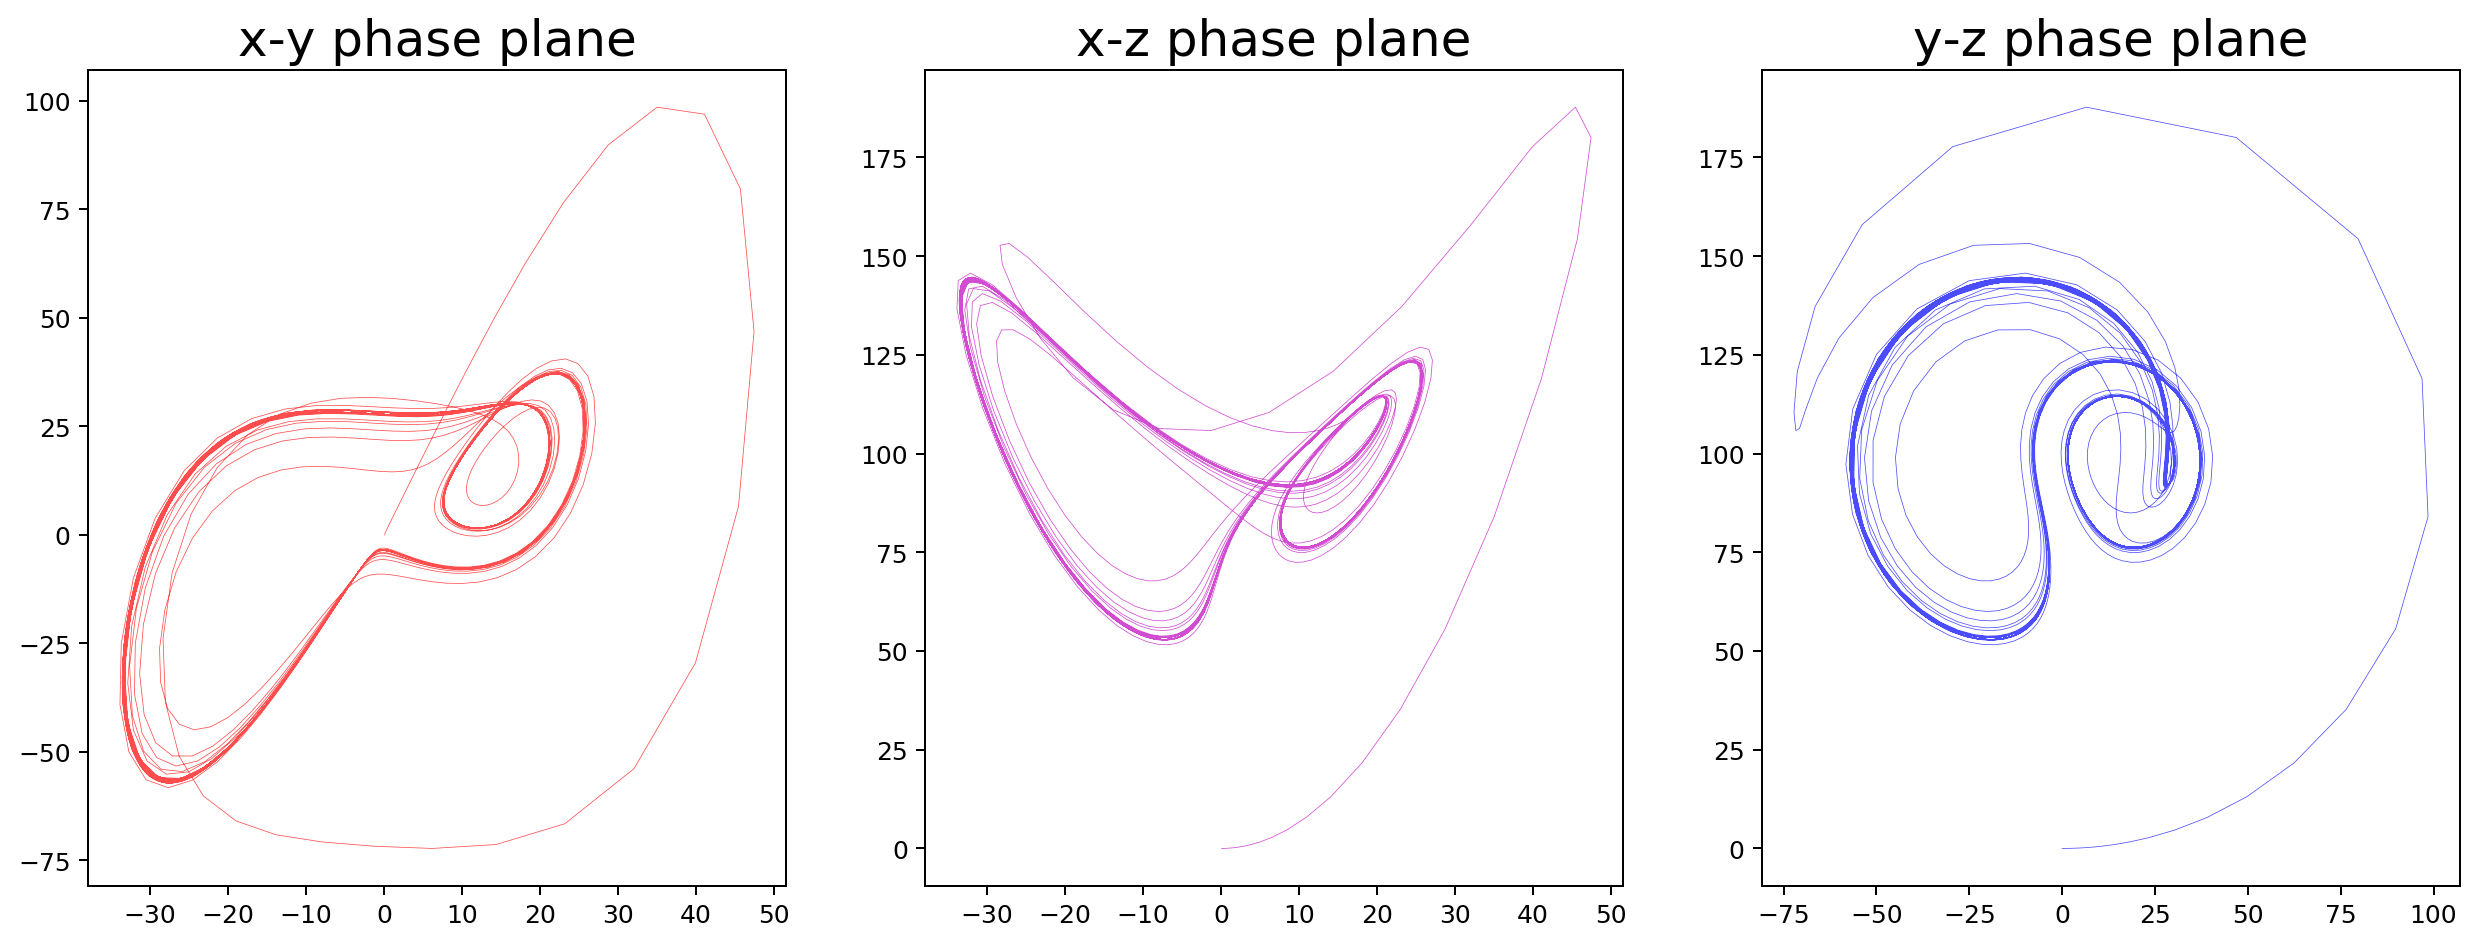
\includegraphics[height=5cm]{lorenz-attractor-phase-plane4.png}
    \end{center}

El comportamiento de cada variable de posición \textit{x(t), y(t), z(t)} con respecto al tiempo:

	\begin{center}
    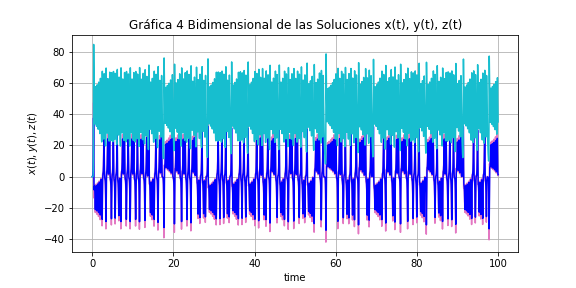
\includegraphics[height=5cm]{2_graficas4.png}
    \end{center}

Como ha pasado en las últimas dos visualizaciones, no podemos distinguir comportamiento de \textit{x(t)} y \textit{y(t)} fácilmente, pero esta vez aunque se proporcione un acercamiento, sus posiciones prevalecen similares:

    \begin{center}
    \centering
    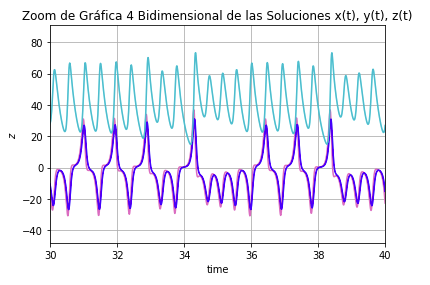
\includegraphics[height=5cm]{2_zoom4.png}
    \end{center}

Cada gráfica del comportamiento de la posición contra el tiempo por separado:

	\begin{center}
    \centering
    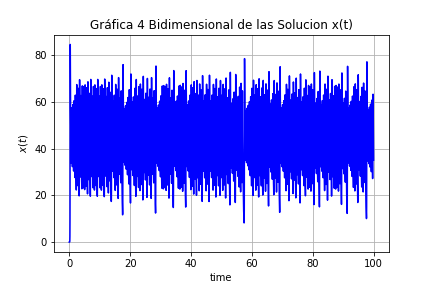
\includegraphics[height=5cm]{2_graficax4.png}
	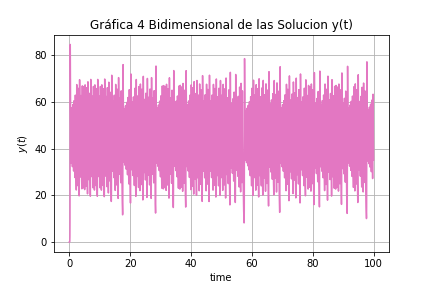
\includegraphics[height=5cm]{2_graficay4.png}
    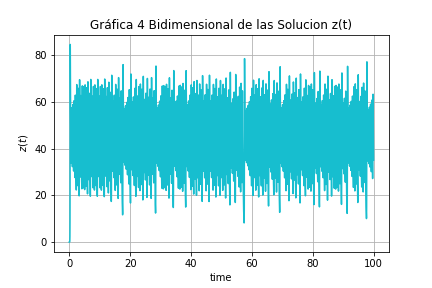
\includegraphics[height=5cm]{2_graficaz4.png}
    \end{center}

\section{Conclusión}
El atractor de Lorenz es un sistema de ecuaciones diferenciales, que a diferencia de la mayoría de las actividades pasadas realizadas con respecto al código, se tenían los diferenciales y no las ecuaciones, por lo cuál primero se tenía que integrar para lograr obtener el sistema y así poder resolver el sistema, encontrando un tipo de caos determinístico.

\section{Bibliografía}
\begin{itemize}
\item El Sistema de Lorenz. Retrieved: 26/04/2018
$http://tesis.uson.mx/digital/tesis/docs/18917/Capitulo4.pdf$
\end{itemize}


\end{document}
